\chapter{Testing and Evaluation}

To be able to answer our research questions of how to improve the performance of
Web services in DIL environments, we developed test setups and environments to
evaluate the proxy. The goal is to measure any possible improvements(or
deterioration) of performance when we use the proxy developed as a part of
this thesis. In this chapter we present how the testing was performed and
finally present the results we obtained.

\section{Introduction}

The proxy is being developed as a prototype for military usage, we therefore
wanted to use a test scenario that resembles actual military usage. For the
purpose of testing we for those reasons used two applications developed by FFI,
programs which allows soldiers in the field to report positions of friendly and
enemy forces back to a headquarter. The soldiers use a simple Web service client
which sends a Web service some sort of data. These applications are W3C Web
services, but as we have previously discussed it is also interesting to look at
RESTful Web services. For testing, we therefore also developed a RESTful Web
service, which does X. Each test case is performed with both a W3C Web services
and RESTful Web services.

Furthermore we performed tests with two setups, first with machine-to-machine
over an Ethernet cable, then over actual military communication equipment. The
usage of actual military equipment allowed us to get as realistic results as
possible. To evaluate how different network properties affects performance, the
tests was performed on networks with different characteristics. The base case
was to test without any intentional limitations to the network and without the
actual usage of the proxy. Then we introduced usage of the proxy and evaluated
it in different types of network types. An infinite number of possible network
combinations exists, so we have in this thesis chosen to focus on five different
network types. These five different types were identified by the task group
IST-118 for DIL-testing and are summarized in \cref{table-network-types}.

\begin{table}[h]
\begin{tabular}{| l | l | l | l | l |}
\hline
  \textbf{Network} & \textbf{Data Rate} & \textbf{Delay} & \textbf{PER} \\ \hline
  Satellite Communication & 250 kbps & 550 ms & 0 \% \\ \hline
  Line of Sight & 2 mbps & 5 ms & 0 \% \\ \hline
  Wireless Fidelity (WiFi) 1 & 2 mbps & 100 ms & 1 \% \\ \hline
  WiFi 2 & 2 mbps & 5 ms & 20 \% \\ \hline
  Combat Net Radio with Forward Error Correction & 9.6 kbps & 100 ms & 1 \% \\ \hline

\end{tabular}
\caption{Different network types}
\label{table-network-types}
\end{table}

\section{Evaluation Tools}

In order to simulate \gls{dil} environments we need some way to control the
properties of the network traffic. In this thesis we use two approaches, the
first one connecting two machines through a third machine. The third machine
will use a component of the linux kernel to control the flow of the network
traffic flowing through it, allowing us to simulate a DIL network. The second
approach involves using actual military equipment in laboratory at FFI. The
benefit of using actual equipment, is that we get as realistic tests as
possible.

\subsection{\glsentrylong{netem}}

Fortunately, the Linux kernel offers a rich set of tools for managing and
manipulating the transmission of packets. \gls{netem} is an enchancement of the
traffic control facilities that allows us to control delay, packet loss and
other characteristics to packets outgoing from a selected network interface.
\Cref{figure-testing-environment} illustrates the setup of this approach.

%Siter man-page om tc-netem
%Siter tldp -> Traffic Control HOWTO

\begin{figure}[h]
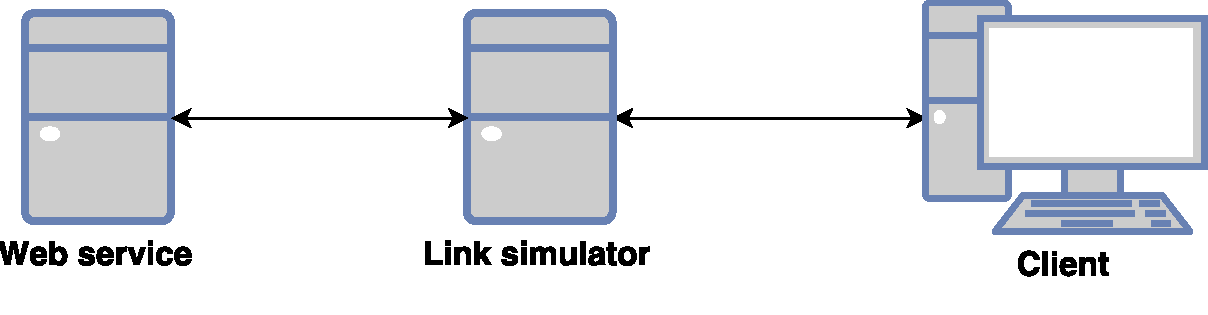
\includegraphics[scale=0.6]{images/testing_environment.pdf}
\caption{Testing environment}
\label{figure-testing-environment}
\end{figure}


\textbf{tc}(traffic control) is a linux program to configure and control the
linux kernels Network scheduler. This program allows us to emulate many of the
network characteristics that DIL has and the different setups are explained in
the coming sections.

\subsubsection{Delays}

NetEm can emulate delays on packets on a specific link.

\begin{lstlisting}[frame=single, caption="Emulating delay"]
  tc qdisc add dev eth0 root netem delay 100ms
\end{lstlisting}

In this example we add a fixed delay on 100 ms to all packets going out of local
Ethernet.

\subsection{Testing on military communication equipment}
Kongsberg radio.


\section{Testing environment}
\label{testing-environment}

The majority of testing was performed on machines located at the FFI-lab at
Kjeller. Although testing on regular machines gives us a indication, to get as
realistic results as possible we also performed tests on military communication
equipment.

\subsection{Using proxies}

In order to enable the applications to tunnel all their HTTP traffic through our
proxy, we needed a way to setup a proxy without altering the applications
themselves. Fortunately, Java provide mechanisms to deal with
proxies\cite{oracle-proxy}. We configured the \gls{jvm} to get the applications
to tunnel all HTTP traffic through our proxy. This is done by setting properties
to the \gls{jvm}:


\begin{lstlisting}[frame=single, caption="Setting a proxy on the \gls{jvm}", label=test]
java -Dhttp.proxyHost=localhost \
-Dhttp.proxyPort=3001 \
-Dhttp.nonProxyHosts= \
-jar target/client.jar
\end{lstlisting}

In \cref{test} the application \textbf{client.jar} is started and all HTTP
traffic will go through the proxy server at localhost on port 3001.

\subsection{Setting up routing}

 The Web service and client are connected to each other through a third
 computer, acting as a router. This machine have two network cards and will
 receive and forward IP packets from the client and Web service. The machines
 are networked together by Ethernet cables.

\paragraph{Configuration}

This section describes how the test setup was performed. The computers running
the client and Web service are connect by an Ethernet cable to the "routing"
machine. Then they are assigned an IP address. This is done by the Linux network
interface administration program \textit{ifconfig}. In \cref{listing-ifconfig}
the Ethernet interface is assigned the IP address 192.168.2.3.

\begin{lstlisting}[frame=single, caption="Configuring a network interface of the router", label=listing-ifconfig]
ifconfig eth0 192.168.2.1 up
\end{lstlisting}


\begin{lstlisting}[frame=single, caption="Configuring a network interface of client", label=listing-ifconfig]
ifconfig eth0 192.168.2.44 up
\end{lstlisting}

\begin{lstlisting}[frame=single, caption="Configuring routing rules for the client", label=listing-ifconfig]
ip route add unicast 192.168.1.0/24 via 192.168.2.1
\end{lstlisting}


\section{Function tests}

The first phase of the testing was performed without any actual intended
limitations to the network. The objective of this testing is to validate that
the proxy is working correctly and have a benchmark to compare other results
with. This phase was again divided into two phases, one without the usage of
proxy and one with the usage of it. This allows us to investigate any potential
overhead associated with the usage of the proxy.

\subsection{Execution}

The Web service client and the service itself was started on separately machines
interconnect through a third machines acting as a router as discussed in
\cref{testing-environment}. However for the first phase, the client and server
did not use any proxy.


\subsection{Results}

\begin{table}[h!]
\begin{tabular}{| l | l | l |}
\hline
  \textbf{Test} & \textbf{Avg. RTT} & \textbf{With compression}\\ \hline
  Without proxy & 117 ms & N/A \\ \hline
  Proxy with HTTP & 148 ms & 93 ms \\ \hline
  Proxy with AMQP & 631 ms & 509 ms \\ \hline
  Proxy with CoAP & 255 ms & 102 ms \\ \hline
\end{tabular}
\caption{W3C Web service results}
\end{table}

\begin{table}[h!]
\begin{tabular}{| l | l | l |}
\hline
  \textbf{Test} & \textbf{Transfer time} & \textbf{With compression}\\ \hline
  Without proxy & 1000 ms & N/A \\ \hline
  Proxy with HTTP & 1200 ms & 1000\\ \hline
  Proxy with AMQP & 1200 ms & 1000\\ \hline
  Proxy with CoAP & 1200 ms & 1000\\ \hline
\end{tabular}
\caption{RESTful Web service results}
\end{table}


\section{DIL Tests - Disconnected}

In this scenario we evaluating the performance with the DIL characteristic
\textit{disconnected}, which refers to the network suddenly going down when the
application is sending data. The objective of this testing is to evaluate how
the proxy manages disconnects.

\subsection{Execution}

Physically removing the Ethernet cable during transmission. 60 seconds?

\subsection{Results}

\begin{table}[h!]
\begin{tabular}{| l | l |}
\hline
  \textbf{Test} & \textbf{Result} \\ \hline
  Without proxy & Timeout \\ \hline
  Proxy with HTTP & Success \\ \hline
  Proxy with AMQP & Success \\ \hline
  Proxy with CoAP & Success \\ \hline
\end{tabular}
\caption{W3C Web service results}
\end{table}

\begin{table}[h!]
\begin{tabular}{| l | l |}
\hline
  \textbf{Test} & \textbf{Result} \\ \hline
  Without proxy & Timeout \\ \hline
  Proxy with HTTP & Success \\ \hline
  Proxy with AMQP & Success \\ \hline
  Proxy with CoAP & Success \\ \hline
\end{tabular}
\caption{RESTful Web service results}
\end{table}

\section{DIL Tests - Intermittent}

\textit{Intermittent} refers to the network connection being lost, but then regained again.

\subsection{Execution}

Disconnect physically, then reconnecting it.

\subsection{Results}

\begin{table}[h!]
\begin{tabular}{| l | l | l | l |}
\hline
  \textbf{Test} & \textbf{10 sec} & \textbf{30 sec} & \textbf{60 sec} \\ \hline
  Without proxy & Timeout & Timeout & Timeout \\ \hline
  Proxy with HTTP & 1400 ms & 40000 & Timeout \\ \hline
  Proxy with AMQP & 1400 ms & 40000 & Timeout \\ \hline
  Proxy with CoAP & 1400 ms & 40000 & Timeout \\ \hline
\end{tabular}
\caption{W3C Web service results}
\end{table}

\begin{table}[h!]
\begin{tabular}{| l | l | l | l |}
\hline
  \textbf{Test} & \textbf{10 sec} & \textbf{30 sec} & \textbf{60 sec} \\ \hline
  Without proxy & 10000 ms & Timeout & Timeout \\ \hline
  Proxy with HTTP & 1200 ms & 12000 & 60000 \\ \hline
  Proxy with AMQP & 1200 ms & 12000 & 60000 \\ \hline
  Proxy with CoAP & 1200 ms & 12000 & 60000 \\ \hline
\end{tabular}
\caption{RESTful Web service results}
\end{table}

\section{DIL Tests - Limited}

The third DIL characteristic \textit{limited} refers to different ways a network
can be limited. This includes high delays, packet loss and low bandwidth. The
different types of networks we want to test were listed in
\cref{table-network-types}. In the following sections the proxy is tested for
each network configuration.


\subsection{Satellite communication}

In this test scenario we emulate \gls{satcom}. Low data rate, high delay.

\paragraph{Results}

\begin{table}[h!]
\begin{tabular}{| l | l | l |}
\hline
  \textbf{Test} & \textbf{Transfer time} & \textbf{With compression}\\ \hline
  Without proxy & 6235 ms & N/A ms \\ \hline
  Proxy with HTTP & X ms & 3504 ms \\ \hline
  Proxy with AMQP & X ms & 24414 ms \\ \hline
  Proxy with CoAP & X ms & 11210 ms \\ \hline
\end{tabular}
\caption{RESTful Web service results}
\end{table}

\subsection{Line-of-Sight}

In this test scenario we emulate so-called \gls{los} networks, which are
characterized by being a radio-based type of network with no physical obstacles
between the nodes in the network. High data rate, low delay and zero error.

\subsection{WiFi 1}

Placeholder.


\subsection{WiFi 2}

Placeholder

\subsection{Combat Net Radio with Forward Error Correction}

Placeholder.

\section{Summary}

In this section the results from the tests are presented. These results lead up
to the discussion and conclusion in the next chapter.
